\documentclass{article}
\usepackage[utf8]{inputenc}
\usepackage{hyperref}
\hypersetup{
    colorlinks=true,
    linkcolor=blue,
    filecolor=magenta,      
    urlcolor=cyan,
    pdftitle={Overleaf Example},
    pdfpagemode=FullScreen,
    }

\title{Residual Connections and Inception Modules}
\author{Tarushii Goel\footnote{This lecture is adapted from Justin Zhang's 2017 lecture on ResNets and Inception}}
\date{2020}


\usepackage[letterpaper, margin=1in]{geometry}
\usepackage{natbib}
\usepackage{graphicx}
\usepackage{amsmath}

\begin{document}

\maketitle

\section{Residual Connections}
\subsection{Motivation}
For many years, the trend in machine learning was to add more layers, since larger networks can capture more complexity (case in point, VGGs). However, one big issue that arises with this approach is the {\bf vanishing gradient}. Since gradients are calculated by multplying partial derivatives, if the partial derivatives are small, as is often the case in practice, the gradients become exponentially smaller, or vanish, as you back propogate to the initial layers to your network. This results in initial layers recieving very small updates. For example, the derivatives of the hyperbolic tangent function are in the range (0,1), so backpropogation through this function will always cause the gradient to decrease. The initial layers train so slowly that the benefit of having them quickly declines. In fact, the initial layers can start to hurt the accuracy of the model. To solve these issues, researchers invented residual connections, which are "skip" connections that fuction as information highways for passing gradient information and prevent a vanishing gradient. 
\begin{center}
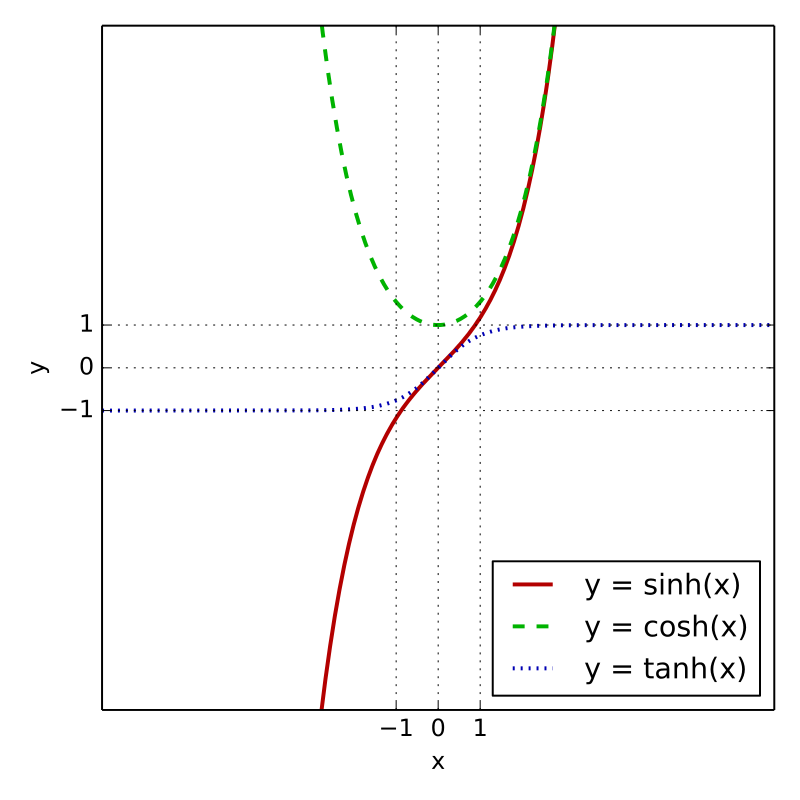
\includegraphics[scale=0.2]{tanh.png}
\end{center}

\subsection{Idea}
\begin{center}
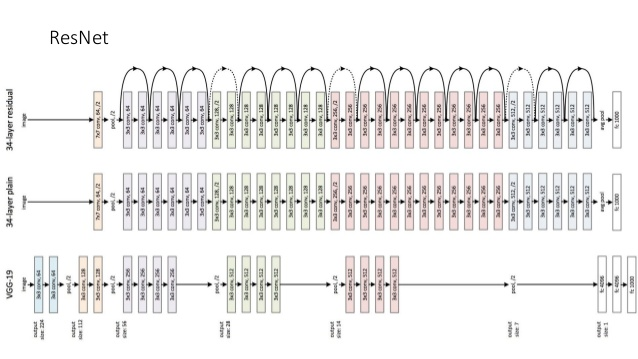
\includegraphics[scale=0.5]{resnet.jpg}
\end{center}
As you can see, ResNet allows for much greater depth than VGG allows. The image above is the smallest conventional size of ResNet. Typical applications use ResNet-50 at least and high-end ones use ResNet-152. The sheer power of these structures has allowed for 92.9 percent accuracy on ImageNet and the usage of training on fancy GPUs with lots of data.

\begin{center}
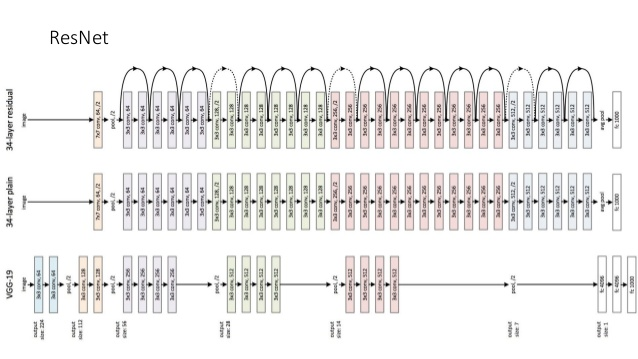
\includegraphics[scale=0.5]{resnet}
\end{center}
To understand the underlying idea behind resiudual connections, let's zoom into one block of a ResNet. The 2 layers shown in the diagram above receive an input, $x$, from the previous layer in the model. We will define the function that we are trying to learn as $H(x)$. In a standard network, we would train this block to learn $H(x)$. However, since this is a residual block, we are instead going to train the model to learn $F(x) := H(x) - x$. $F(x)$ is the residual. The main hypothesis of Residual Networks (one that has been shown to be true in practice) is that $F(x)$ is an easier function to learn than $H(x)$. \\

There are a number of observations you should note about shortcut connections:
\begin{enumerate}
    	\item They do not add extra parameters, and thus no extra computational complexity.
    	\item Since nonlinearities are universal approximators of functions, clearly the residual unit is also a universal approximator.
	\item The degradation problem suggests that the solvers might have difficulties in approximating identity mappings with multiple nonlinear layers. However, with the residual learning formulation, in situations where identity mappings are optimal (or close to optimal), the solvers may simply drive the weights of the multiple nonlinear layers toward zero to approach identity mappings. This means that we can reasonably expect that a deeper residual network will never be worse that its shallower counterpart.
\end{enumerate}

\subsection{Residual Blocks, More Formally}
The residual block protrayed above is defined as:
$$ y = F(x; W_i) + x$$
where $x$ is the input into the block and $y$ is the output of the block. F is the function applied by the 2 stacked non-linear layers, $ F = W_2 \sigma(W_1 x) $ (biases are ommited for notational convenience), and $\sigma$ is the ReLU activation. A second non-linearity is applied after the addition, $\sigma(y)$. $F(x)$ may vary, depending on the number layers you have, and may produce an output of different dimensions than $x$. In this case, we can perform a linear projection $W_s$ on $x$: $ y = F(x; W_i) + W_s x$. This is sufficient to solve the degradation problem. Other methods (zero-padding, for instance) can also work, but the empirical difference between these methods is very small.

\section{Inception}
\begin{center}
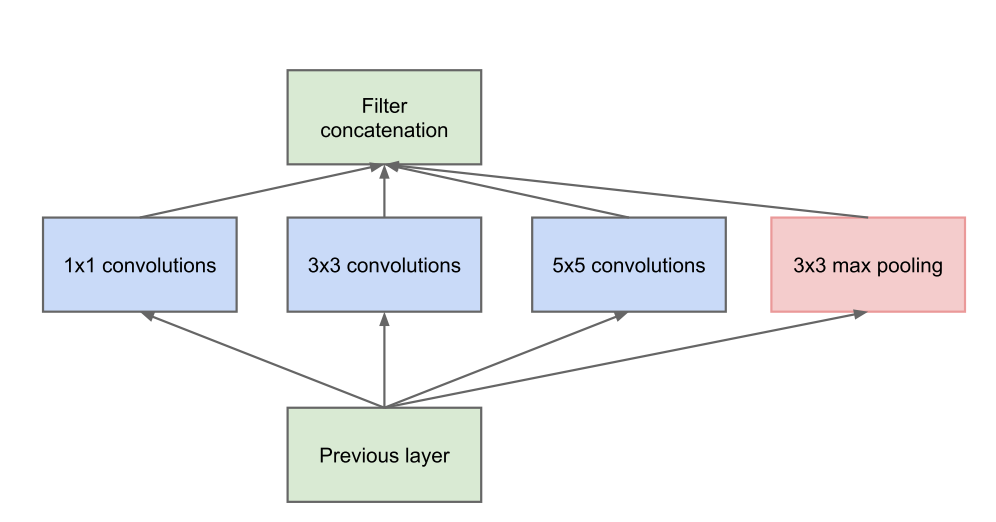
\includegraphics[scale=0.5]{inception}
\end{center}
\subsection{Overview}
Another major improvement made in recent years in image classification is the use of multiple parallel layers in each residual node. Each of these sets of layers, as seen in the image above, contains different filter sizes, allowing for a varying sizes of features to be extracted, the removing the need to optimize filter size as another hyperparameter. These innovations have brought about Inception-ResNet structures capable of producing results more accurate than humans on image classification.

\subsection{Specifics}
    The idea of Inception layers was based off the ``we need to go deeper" internet meme. This automatically gives it more legitimacy over general neural networks, which were modeled after the brain, and reinforcement learning, which was modeled after operant conditioning.
    
    ``Deeper," in this context, refers to two things: a new level of network organization and literal deeper networks. 
    
    To understand the Inception architecture, consider a fundamental trade-off of convolutional networks: the most straightforward way to improve performance is to increase network size. This comes with two drawbacks: overfitting (due to more parameters) and a large drop in performance. Sparsely connected architectures could theoretically solve this as well as better approximate biological processes and single out discrimanatory features, but technical details prevent modern computers from efficiently doing numerical computations with sparse matrices.
    
    The Inception architecture seeks to use varying filter sizes (allowing the model to choose the optimal one, or even combine them) while trying to mimic the result of a sparse structure. 
    
    \begin{center}
    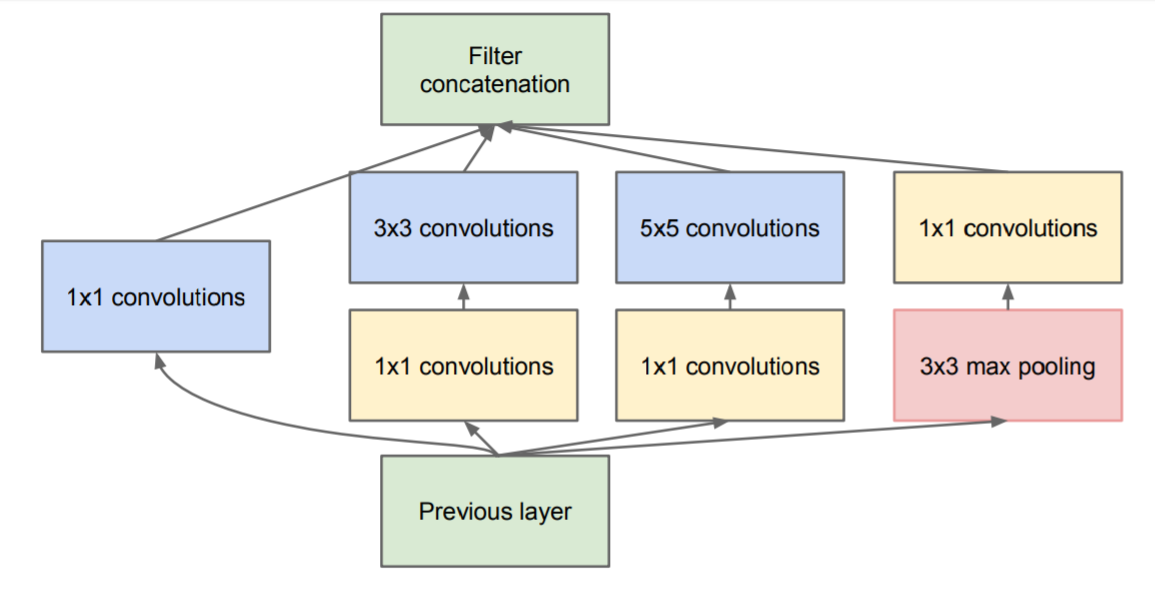
\includegraphics[scale=0.5]{inception2}
    \end{center}
    
    This revised architecture uses dimensionality reduction to make the inception module more efficient and to keep representations of data sparse (i.e. dense convolutions are used with sparser data). Specifically, max pooling (for obvious reasons) and 1x1 convolutions are used.
    
    These 1x1 convolutions do the following:
    \begin{enumerate}
        \item Make the network deeper
        \item Reduce dimensions (the number of feature maps)
        \item Add more non-linearities (ReLU after the 1x1 convolutions)
    \end{enumerate}
    
 Generally, Inception modules are only used in the beginning of a convolutional network, for memory efficiency. 
    
   
\section{Sources}
\begin{itemize}
	\item \href{https://tjmachinelearning.com/lectures/1718/deepconv/deepconv.pdf}{Justin Zhang's Lecture} 
	\item \href{https://en.wikipedia.org/wiki/Vanishing_gradient_problem}{Vanishing Gradient Wikipedia Article}
	\item \href{https://arxiv.org/pdf/1512.03385v1.pdf}{ResNet Paper}
 	\item \href{https://www.coursera.org/lecture/convolutional-neural-networks/inception-network-motivation-5WIZm}{Andrew Ng's Video on Inception}
	\item \href{https://github.com/pytorch/vision/blob/7c077f6a986f05383bcb86b535aedb5a63dd5c4b/torchvision/models/resnet.py#L118}{ResNet Code}
\end{itemize}

\end{document}
